\documentclass{article}
\usepackage{graphicx,fancyhdr,amsmath,amssymb,amsthm,subfig,url,hyperref}
\usepackage[margin=1in]{geometry}

% Added by Hendra
\usepackage{cancel}
\usepackage{natbib}
\usepackage{mathtools}
\usepackage[shortlabels]{enumitem}
\usepackage{hyperref}


\DeclarePairedDelimiter\abs{\lvert}{\rvert}%
\DeclarePairedDelimiter\norm{\lVert}{\rVert}%


%----------------------- Macros and Definitions --------------------------

%%% FILL THIS OUT
\newcommand{\studentname}{Jane Doe}
\newcommand{\suid}{janedoe}
\newcommand{\exerciseset}{Homework}
%%% END


\renewcommand{\theenumi}{\bf \Alph{enumi}}

\theoremstyle{plain}
\newtheorem{theorem}{Theorem}
\newtheorem{lemma}[theorem]{Lemma}


\graphicspath{{figures/}}

%-------------------------------- Title ----------------------------------

\title{Usulan Soal Pra-KSN} 
\author{Hendra Bunyamin \\ {\small Email: hendra.bunyamin@it.maranatha.edu}}
%--------------------------------- Text ----------------------------------

\begin{document}
\maketitle

%	\begin{enumerate}[-,topsep=0pt, nosep,label=\arabic*. ]
%		\item \textit{history data} adalah data numerik;
%		\item asumsi bahwa beberapa aspek dari pola terdahulu akan berlanjut di masa depan.
%	\end{enumerate}


% ========================
%   Soal 1: Algoritma Dijkstra    
% ========================
\section*{Problem 1}
Diketahui suatu peta dari enam kota ($a$, $b$, $c$, $d$, $e$, $z$) yang dilambangkan dengan simpul atau titik dan jalan raya yang menghubungkan antar kota dengan sisi atau garis seperti pada Figure~\ref{fig:peta-enam-kota}. Panjang jalan raya dinyatakan dalam bentuk angka; contohnya, panjang jalan raya yang menghubungkan kota $b$ dan $e$ adalah $5$. 

\begin{figure}[!ht]
	\centering
	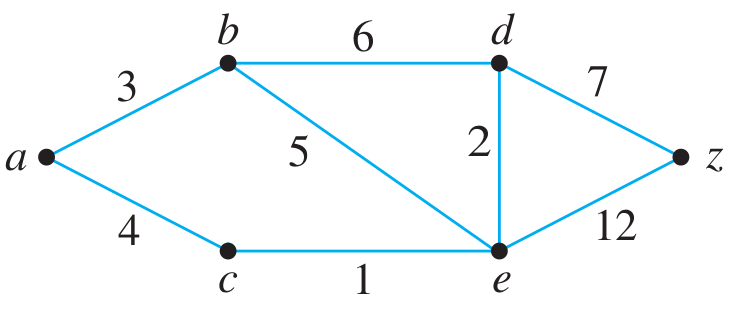
\includegraphics[scale=.25]{images/dijkstra}
	\caption{Peta dari enam kota}
	\label{fig:peta-enam-kota}
\end{figure}

\noindent Anda hendak berangkat dari kota $a$ menuju kota $z$ dan untuk menghemat waktu dan biaya bensin, anda hendak merancang rute perjalanan dari kota $a$ menuju kota $z$ yang sependek mungkin.\\
Berapakah panjang rute terpendek yang dapat dibentuk dari kota $a$ menuju kota $z$?
	\begin{enumerate}[-,topsep=0pt, nosep,label=\alph*. ]
		\item 14
		\item 13
		\item 12
		\item 15
		\item 11
	\end{enumerate}


\bigskip
\noindent \textbf{Jawab}: \textbf{a}

\newpage
\section*{Problem 2}
Terdapat beberapa buah kota yang terhubung dengan penerbangan satu arah (arah penerbangan ditunjukkan dengan tanda panah) sebagai pada Figure~\ref{fig:jadwal-penerbangan}.

\begin{figure}[!ht]
\centering
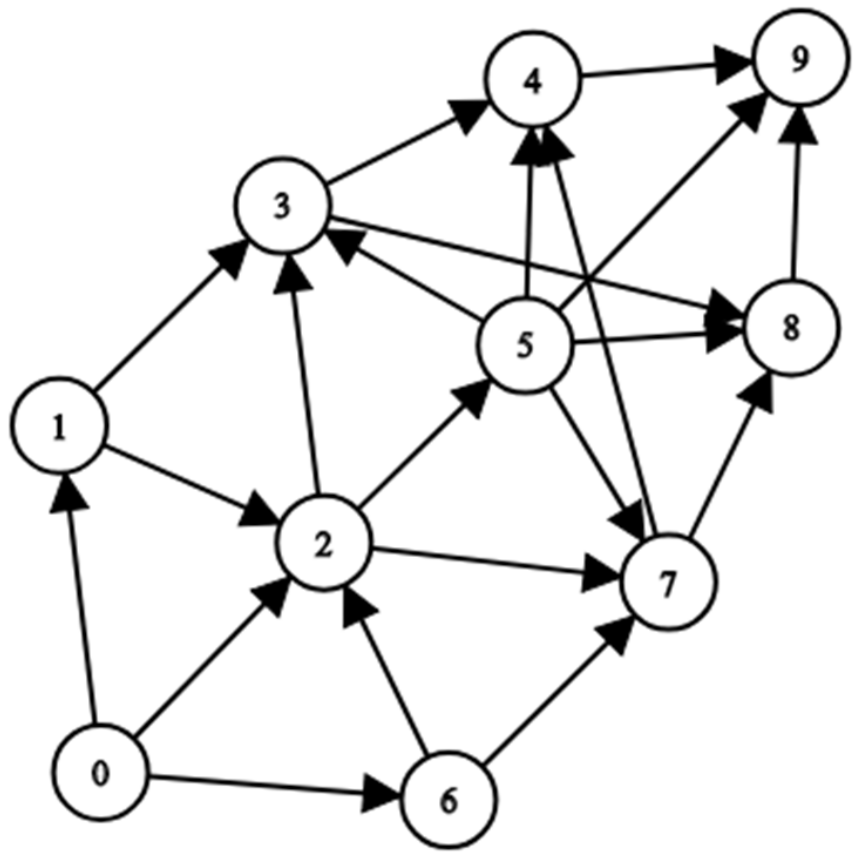
\includegraphics[scale=.225]{images/problem-2-dan-3}
\caption{Jadwal penerbangan dengan tanda panah adalah arah penerbangan}
\label{fig:jadwal-penerbangan} 
\end{figure}

\noindent Jika diketahui Pak Dennis melakukan perjalanan dari Kota-0 ke Kota-9 melewati tepat 4 penerbangan, berapa banyak kemungkinan rute berbeda yang bisa diambil?
	\begin{enumerate}[-,topsep=0pt, nosep,label=\alph*. ]
		\item 14
		\item 13
		\item 12
		\item 15
		\item 11
	\end{enumerate}

\bigskip
\noindent \textbf{Jawab}: \textbf{c}

\newpage
\section*{Problem 3}
Terdapat beberapa buah kota yang terhubung dengan penerbangan satu arah (arah penerbangan ditunjukkan dengan tanda panah) sebagai pada Figure~\ref{fig:jadwal-penerbangan-soal-3}.

\begin{figure}[!ht]
\centering
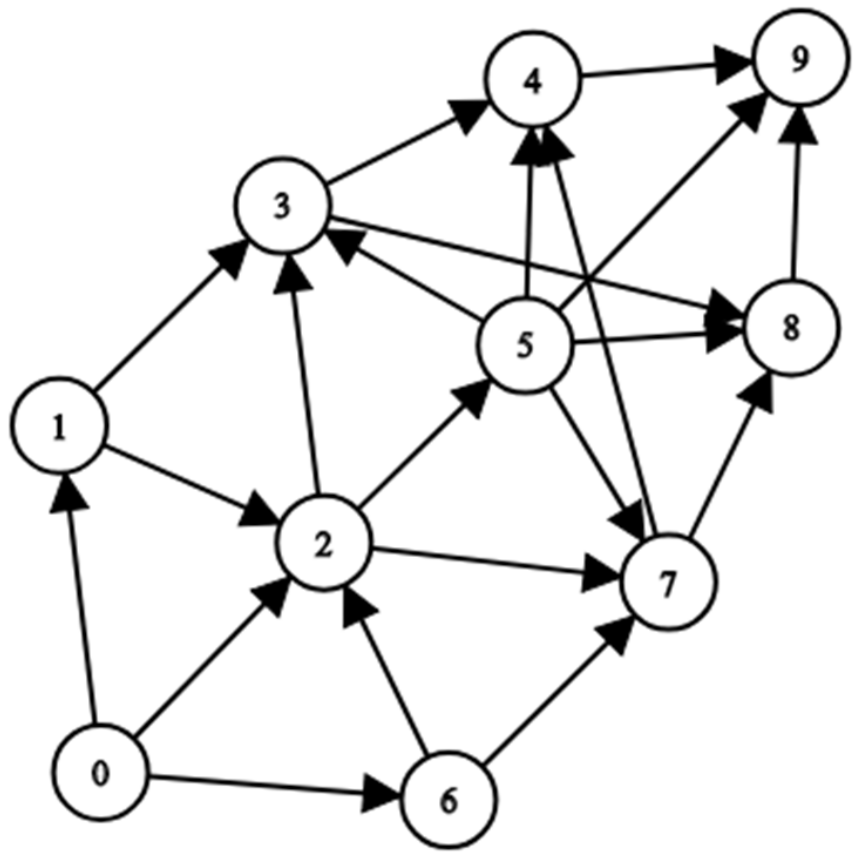
\includegraphics[scale=.225]{images/problem-2-dan-3}
\caption{Jadwal penerbangan dengan tanda panah adalah arah penerbangan}
\label{fig:jadwal-penerbangan-soal-3} 
\end{figure}

\noindent Untuk menghindari kemungkinan cuaca buruk, beberapa rute penerbangan akan dibatalkan. Berapa rute penerbangan minimal yang harus ditutup sedemikian sehingga banyaknya rute yang bisa diambil dari Kota-0 ke Kota-9 masih tersisa tepat 2 kemungkinan rute?
	\begin{enumerate}[-,topsep=0pt, nosep,label=\alph*. ]
		\item 14
		\item 13
		\item 12
		\item 15
		\item 11
	\end{enumerate}

\bigskip
\noindent \textbf{Jawab}: \textbf{e}

\newpage
\section*{Problem 4}
Pak Dennis memiliki array $A$ dengan panjang $N$. Indeks pada $A$ dimulai dari $0$ sampai dengan $N-1$. Nilai elemen $A$ pada indeks $i$ bernilai $i \oplus (i + 1) \oplus (i + 2) \oplus \ldots \oplus (N-1)$. Nilai elemen A pada indeks $N-1$ bernilai $N-1$.

\bigskip
\noindent Catatan: $\oplus$ adalah operasi XOR (\textit{Exclusive} OR) biner pada bilangan bulat desimal. Sebagai contoh,

\begin{equation*}
5 \oplus 3 \, (\text{desimal}) = 101 \oplus 011 \, (\text{biner}) = 110 \, (\text{biner}) = 6 \, (\text{desimal}). 
\end{equation*}
Pak Dennis merupakan orang yang sangat penasaran, karena itu beliau membuat fungsi $F(N)$, yang mengembalikan nilai dari $A[0] + A[1] + \ldots + A[N - 2] + A[N - 1]$. 

\bigskip
\noindent Sebagai contoh, apabila $N=4$, maka
\begin{align*}
A[0] &= 0 \oplus 1 \oplus 2 \oplus 3 = 0 \\
A[1] &= 1 \oplus 2 \oplus 3 = 0 \\
A[2] &= 2 \oplus 3 = 1 \\
A[3] &= 3 
\end{align*}
Karena itu,
\begin{equation*}
	F(N) = A[0] + A[1] + A[2] + A[3] = 0 + 0 + 1 + 3 = 4.
\end{equation*}
Berapakah nilai dari $F(N)$ apabila $N=12$?

	\begin{enumerate}[-,topsep=0pt, nosep,label=\alph*. ]
		\item 36
		\item 24
		\item 12
		\item 48
		\item 60
	\end{enumerate}

\bigskip
\noindent \textbf{Jawab}: \textbf{a}

\newpage
\section*{Problem 5}
Pak Dennis memiliki array $A$ dengan panjang $N$. Indeks pada $A$ dimulai dari $0$ sampai dengan $N-1$. Nilai elemen $A$ pada indeks $i$ bernilai $i \oplus (i + 1) \oplus (i + 2) \oplus \ldots \oplus (N-1)$. Nilai elemen A pada indeks $N-1$ bernilai $N-1$.

\bigskip
\noindent Catatan: $\oplus$ adalah operasi XOR (\textit{Exclusive} OR) biner pada bilangan bulat desimal. Sebagai contoh,

\begin{equation*}
5 \oplus 3 \, (\text{desimal}) = 101 \oplus 011 \, (\text{biner}) = 110 \, (\text{biner}) = 6 \, (\text{desimal}). 
\end{equation*}
Pak Dennis merupakan orang yang sangat penasaran, karena itu beliau membuat fungsi $F(N)$, yang mengembalikan nilai dari $A[0] + A[1] + \ldots + A[N - 2] + A[N - 1]$. 

\bigskip
\noindent Sebagai contoh, apabila $N=4$, maka
\begin{align*}
A[0] &= 0 \oplus 1 \oplus 2 \oplus 3 = 0 \\
A[1] &= 1 \oplus 2 \oplus 3 = 0 \\
A[2] &= 2 \oplus 3 = 1 \\
A[3] &= 3 
\end{align*}
Karena itu,
\begin{equation*}
	F(N) = A[0] + A[1] + A[2] + A[3] = 0 + 0 + 1 + 3 = 4.
\end{equation*}
Berapakah nilai dari $F(N)$ apabila $N=200$?

	\begin{enumerate}[-,topsep=0pt, nosep,label=\alph*. ]
		\item 5000
		\item 10000
		\item 15000
		\item 20000
		\item 25000
	\end{enumerate}

\bigskip
\noindent \textbf{Jawab}: \textbf{b}

\newpage
\section*{Problem 6}
Andaikan anda mengunjungi suatu pulau yang dihuni oleh \textbf{ksatria} yang selalu mengatakan yang sebenarnya, \textbf{pengecoh} yang selalu berbohong, dan \textbf{pelawak} yang dapat berbohong atau mengatakan yang sebenarnya. 

\bigskip
\noindent Anda bertemu tiga penghuni pulau yang bernama Ellis, Farin, dan Gobi. Mereka masing-masing mengetahui profesi teman-temannya (apakah ksatria, pengecoh, atau pelawak?) dan membuat pernyataan-pernyataan sebagai berikut:

\bigskip
\noindent \begin{tabular}{ll}
	Ellis &: Farin adalah seorang pelawak \\
	Farin &: Gobi adalah seorang pelawak \\
	Gobi  &: Ellis adalah seorang pelawak.
\end{tabular} 

\bigskip
\noindent Jika terdapat tepat satu pelawak, berapakah banyak ksatria di antara tiga penghuni tersebut?

	\begin{enumerate}[-,topsep=0pt, nosep,label=\alph*. ]
		\item 0
		\item 1
		\item 2
		\item 3
		\item Tidak dapat ditentukan karena kurang informasi
	\end{enumerate}

\bigskip
\noindent \textbf{Jawab}: \textbf{b}

\newpage
\section*{Problem 7}
Terdapat 3 kotak harta karun dan tepat satu dari tiga kotak tersebut menyimpan emas. Emas akan diberikan kepada anda apabila anda dapat memilih kotak harta karun yang tepat menyimpan emas tersebut! Pada setiap kotak harta karun terdapat satu pernyataan dan tepat satu pernyataan saja yang benar.

\bigskip
\noindent \begin{tabular}{ll}
	Tulisan di Kotak 1 &: Emas ada di kotak ini \\
	Tulisan di Kotak 2 &: Emas tidak ada di kotak ini \\
	Tulisan di Kotak 3 &: Emas tidak ada di Kotak 1.
\end{tabular} 

\bigskip
\noindent Kotak manakah yang menyimpan emas?

	\begin{enumerate}[-,topsep=0pt, nosep,label=\alph*. ]
		\item Kotak 1
		\item Kotak 2
		\item Kotak 3
		\item Antara Kotak 1 atau Kotak 3
		\item Tidak dapat ditentukan karena kurang informasi
	\end{enumerate}

\bigskip
\noindent \textbf{Jawab}: \textbf{b}

\newpage
\section*{Problem 8}
Anda mempunyai empat kotak yang tertutup seperti berikut:

\begin{figure}[!ht]
	\centering
	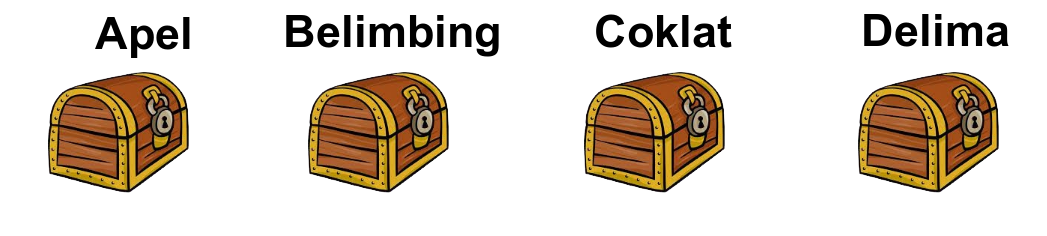
\includegraphics[scale=.25]{images/soal-nomor-9}
\end{figure}

\noindent Anda mengetahui keempat jenis makanan yang ada di dalam setiap kotak dan setiap kotak hanya memuat satu jenis makanan. Anda juga tahu bahwa hanya ada satu kotak yang diberi label secara benar.

\bigskip
\noindent Berapakah \textbf{minimum banyak kotak} yang perlu dibuka agar anda dapat menentukan kotak mana yang diberi label secara benar \textbf{dengan pasti}? (Catatan: \textbf{dengan pasti} berarti berlaku untuk semua skenario, jadi anda tidak dapat berasumsi ada keberuntungan.) 

	\begin{enumerate}[-,topsep=0pt, nosep,label=\alph*. ]
		\item 1
		\item 2
		\item 3
		\item 4
		\item Tidak dapat ditentukan karena kurang informasi
	\end{enumerate}

\bigskip
\noindent \textbf{Jawab}: \textbf{b}

\newpage
\section*{Problem 9}
Di hadapan anda terdapat 3 kotak yang berisi sejumlah koin yang merupakan kombinasi antara koin emas dan perak. Masing-masing kotak memiliki label di atasnya yang menunjukkan berapa banyak koin di dalam kotaknya:

\begin{figure}[!ht]
	\centering
	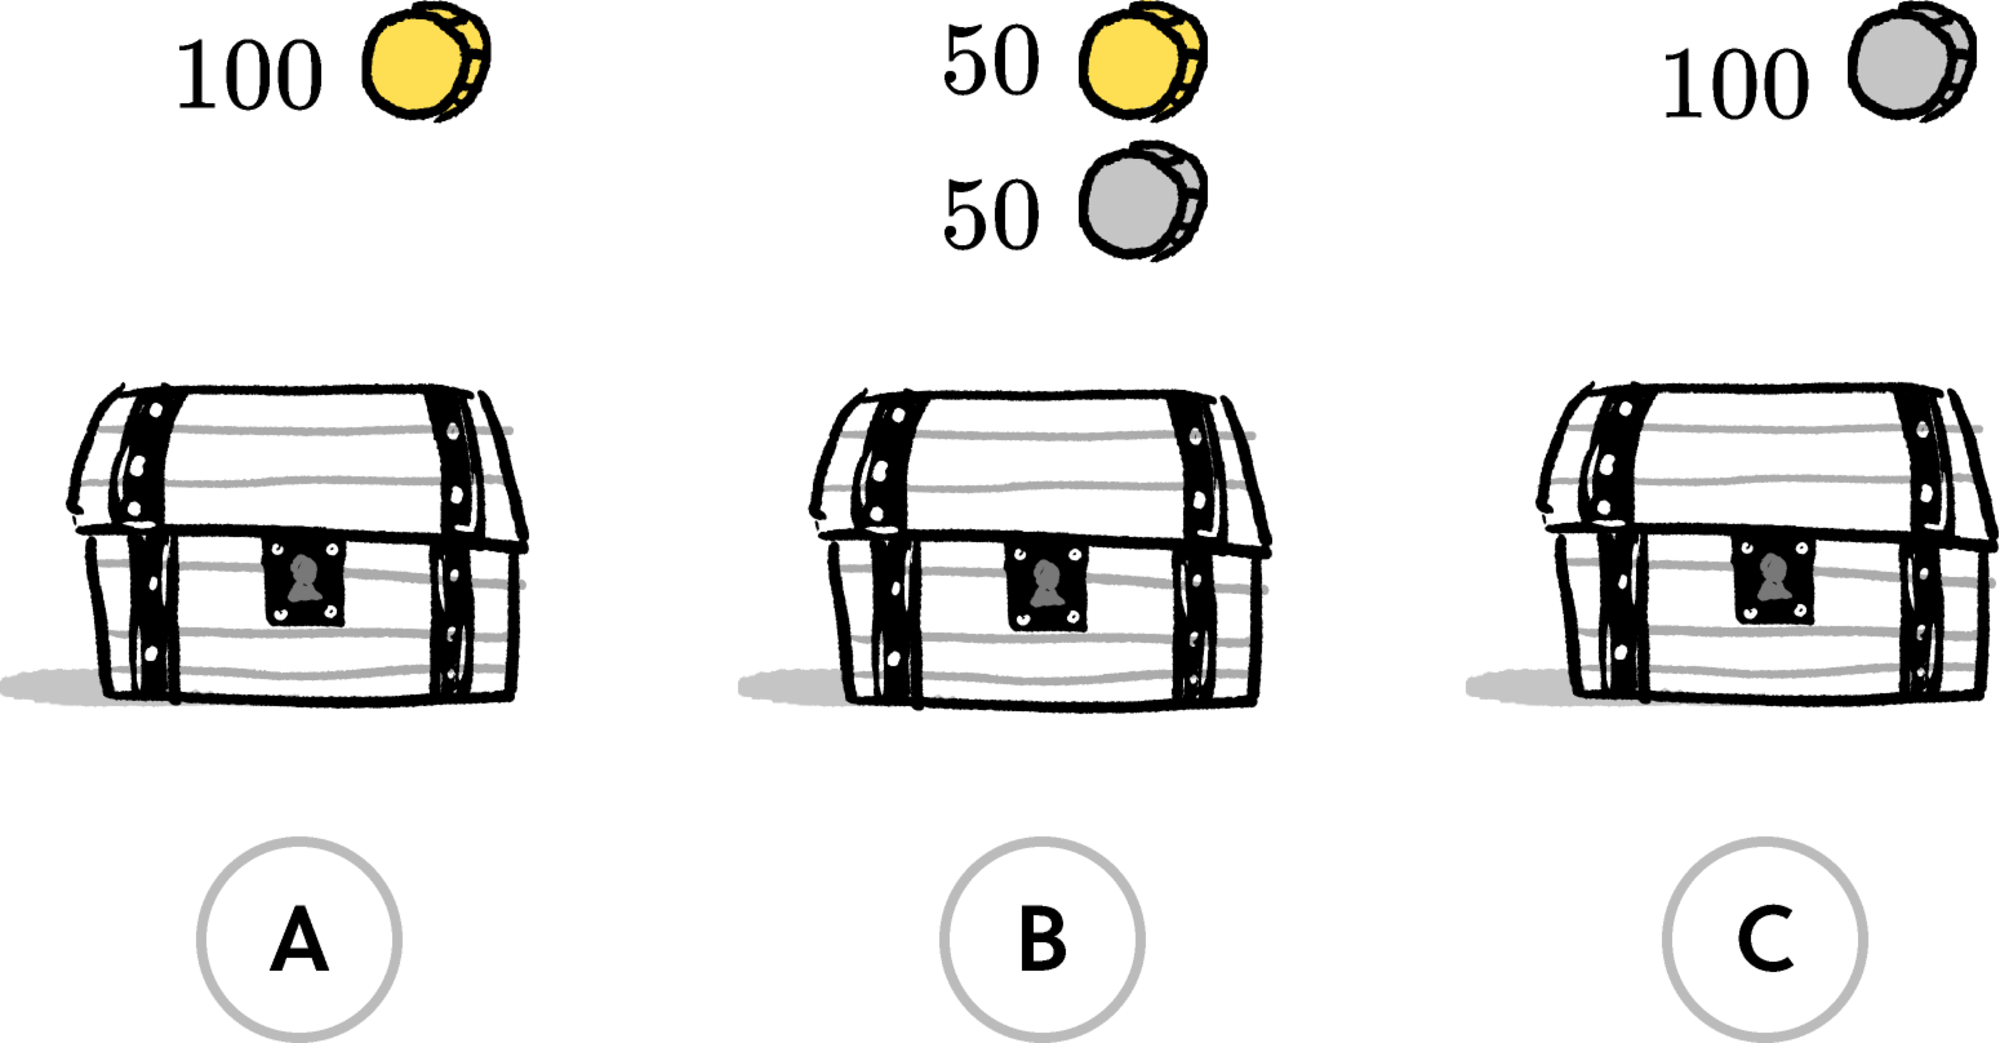
\includegraphics[scale=.12]{images/brilliant}
	\caption{Tiga kotak (gambar ini diambil dari \href{https://brilliant.org}{\textbf{brilliant.org}})}
\end{figure}

\noindent \textbf{Setiap label untuk setiap kotak salah penempatannya}. Setiap label di atas kotak menjelaskan isi dari setiap kotak yang berbeda. \textbf{Untuk menentukan kotak mana yang menyimpan 100 koin emas}, anda dizinkan untuk mengambil satu koin secara acak dari satu kotak yang anda pilih.

\bigskip
\noindent Kotak manakah yang akan anda pilih pertama kali untuk diambil satu koinnya? \\ 
(\textbf{Catatan}: Mengambil satu koin secara acak dari suatu kotak adalah untuk memastikan bahwa 100 koin emas ada di kotak tersebut. Kotak yang anda pilih pertama kali tidaklah harus merupakan kotak yang berisi 100 koin emas. Anda memilih kotak pertama hanya untuk memastikan kotak mana yang berisi 100 koin di dalamnya).

	\begin{enumerate}[-,topsep=0pt, nosep,label=\alph*. ]
		\item Kotak A
		\item Kotak B
		\item Kotak C
		\item Kotak A atau Kotak C
		\item Tidak dapat ditentukan karena kurang informasi
	\end{enumerate}

\bigskip
\noindent \textbf{Jawab}: \textbf{b}


\newpage
\section*{Problem 10}
Untuk mengembangkan usaha peternakannya, Pak Dennis juga akan memelihara ayam selain bebek-bebeknya. Setiap hari, Pak Dennis akan menambah jumlah hewan ternaknya dengan membeli ke toko bebek atau toko ayam secara berselang-seling. Sebagai contoh, apabila kemarin ia pergi ke toko bebek maka hari ini ia akan pergi ke toko ayam. Pak Dennis juga memiliki sebuah aturan pembelian:
	\begin{itemize}[-,topsep=0pt, nosep]
		\item apabila kemarin ia membeli $x$ ekor bebek, maka hari ini ia akan membeli $2x$ ekor ayam;
		\item apabila kemarin ia membeli $y$ ekor ayam, maka hari ini ia akan membeli $3y$ ekor bebek.
	\end{itemize}

\bigskip
\noindent Tentukan hewan ke-1000 yang Pak Dennis beli jika hari pertama dia membeli seekor bebek!

	\begin{enumerate}[-,topsep=0pt, nosep,label=\alph*. ]
		\item Bebek
		\item Ayam
		\item Bisa bebek atau ayam
		\item Pak Dennis membeli piaraan baru, yaitu kambing
		\item Tidak dapat ditentukan karena kurang informasi
	\end{enumerate}

\bigskip
\noindent \textbf{Jawab}: \textbf{a}









\bibliographystyle{apalike}
\bibliography{references}

\end{document}
